\documentclass[a4paper]{article}
\addtolength{\hoffset}{-2.25cm}
\addtolength{\textwidth}{4.5cm}
\addtolength{\voffset}{-3.25cm}
\addtolength{\textheight}{5cm}
\setlength{\parskip}{0pt}
\setlength{\parindent}{0in}

\usepackage[square,sort,comma,numbers]{natbib}
\usepackage{blindtext} % Package to generate dummy text
\usepackage{charter} % Use the Charter font
\usepackage[utf8]{inputenc} % Use UTF-8 encoding
\usepackage{microtype} % Slightly tweak font spacing for aesthetics
\usepackage{amsthm, amsmath, amssymb} % Mathematical typesetting
\usepackage{float} % Improved interface for floating objects
\usepackage{hyperref} % For hyperlinks in the PDF
\usepackage{graphicx, multicol} % Enhanced support for graphics
\usepackage{xcolor} % Driver-independent color extensions
\usepackage{pseudocode} % Environment for specifying algorithms in a natural way
\usepackage[mmddyy]{datetime} % Uses YEAR-MONTH-DAY format for dates

\usepackage{fancyhdr} % Headers and footers
\pagestyle{fancy} % All pages have headers and footers
\fancyhead{}\renewcommand{\headrulewidth}{0pt} % Blank out the default header
\fancyfoot[L]{} % Custom footer text
\fancyfoot[C]{} % Custom footer text
\fancyfoot[R]{\thepage} % Custom footer text
\newcommand{\note}[1]{\marginpar{\scriptsize \textcolor{red}{#1}}} % Enables comments in red on margin

\DeclareMathOperator*{\argmin}{arg\,min}

%----------------------------------------------------------------------------------------

\newcommand{\yourname}{Balthazar Neveu}
\newcommand{\youremail}{balthazarneveu@gmail.com}
\newcommand{\assignmentnumber}{5}

\begin{document}

\fancyhead[C]{}
\hrule \medskip
\begin{minipage}{0.295\textwidth} 
\raggedright
\footnotesize
\yourname \hfill\\
\youremail
\end{minipage}
\begin{minipage}{0.4\textwidth} 
\centering 
\large 
Lab session \# \assignmentnumber\\ 
\normalsize 
ALTEGRAD 2023\\ 
\end{minipage}
\begin{minipage}{0.295\textwidth} 
\raggedleft
\today\hfill\\
\end{minipage}
\medskip\hrule 
\bigskip


\section*{Code}

More info:
\href{https://github.com/balthazarneveu/MVA23_ALTEGRAD/#readme}{MVA ALTEGRAD Balthazar Neveu on Github}

\section{Unsupervised node embeddings using Deepwalk}

We're trying to construct meaningful embeddings for a graph made of crawled french websites.

\begin{itemize}
    \item Number of nodes: 33226 . Each node is a website link.
    \item Number of edges: 354529 . Edges means the presence of hyperlinks between 2 websites.
    \item Dimension of embeddings of Word2Vec: 128
    \item Random walk length = 20
    \item At each node, $n_{walks}=10$ will be pre-stored.
\end{itemize}

\subsection*{Task 1 \& 2: Details on random walks sampling implementations}
Unexpectedly, initial naïve implementation took way too much time. 
Profiling led me to spot two bottlenecks:
\begin{itemize}
    \item I should not use \textit{np.random.choice} but rather \textit{random.randint} 
    to sample the next node in the walk
among neighbors.
    \item In addition, I used a dictionary to pre-store the neighbors instead of using the remove redundant calls to \textit{list(G.neighbors(node))}
    \item In this dataset, nodes are not indexes (e.g. integers) but string (hyperlinks).
    I tried to relabel to ints but it didn't really sped up and addressing the first two points was enough.
\end{itemize}

\begin{verbatim}
# Create a mapping from strings to integers
node_mapping = {node: i for i, node in enumerate(G.nodes())}

# Create a reverse mapping if you need to convert back to strings later
reverse_mapping = {i: node for node, i in node_mapping.items()}
G_int = nx.relabel_nodes(G, node_mapping)
\end{verbatim}

\subsection*{Task 4 : Node embdeddings visualization}
Refer to  \ref{fig:node_embeddings}
\begin{figure}[ht]
    \centering
    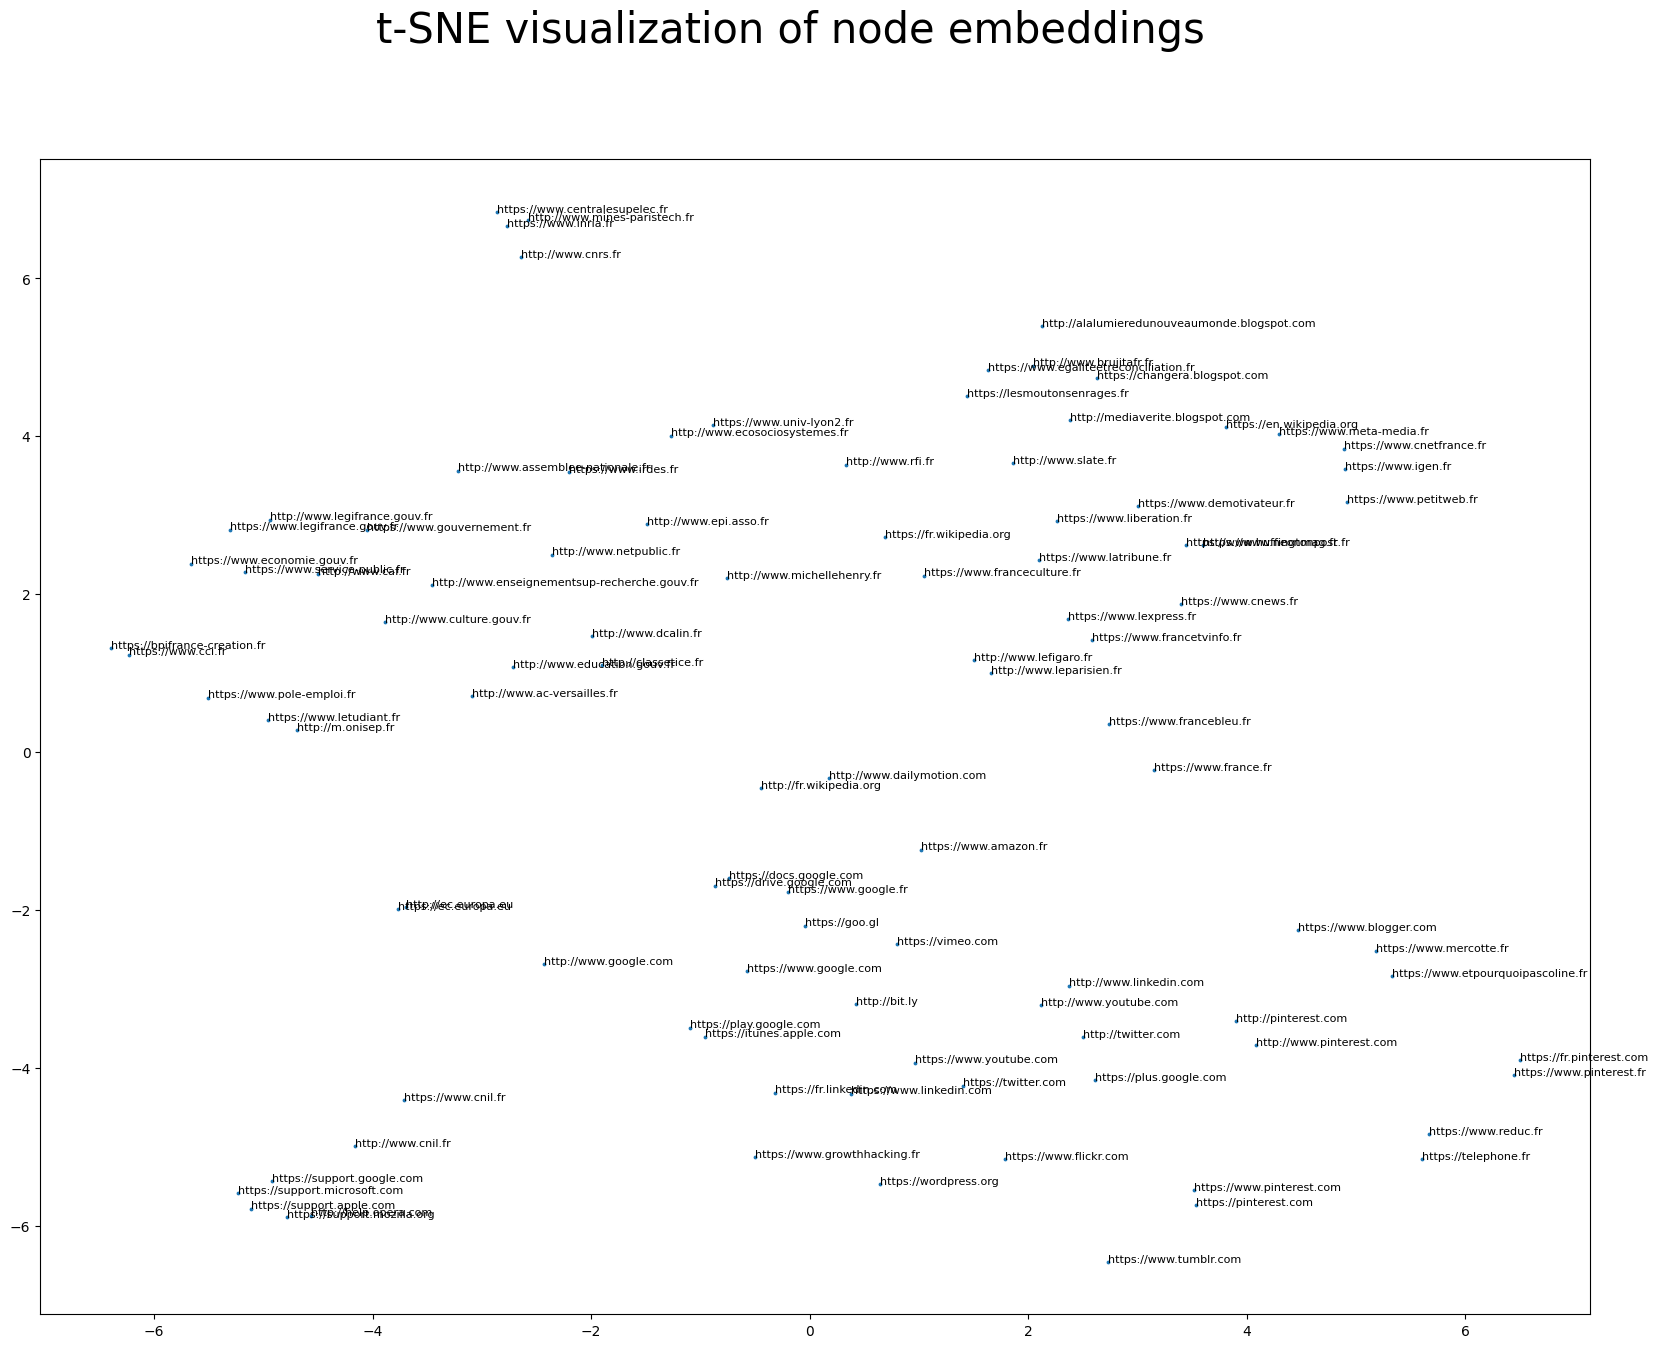
\includegraphics[width=0.6\textwidth]{figures/tSNE_node_embeddings.png}
    \caption{t-SNE is used on the high (128) dimensional node embeddings to reduce dimensionality to 2D coordinates,
    which allows visualization of a few samples (here $n=100$) - embdeddings look relevant from the name of the website e.g.
    Pinterest, Tumblr, Wordpress appear in the same location for instance.}
    \label{fig:node_embeddings}
\end{figure}

\break
\subsection*{Question 1}

\begin{figure}[ht]
    \centering
    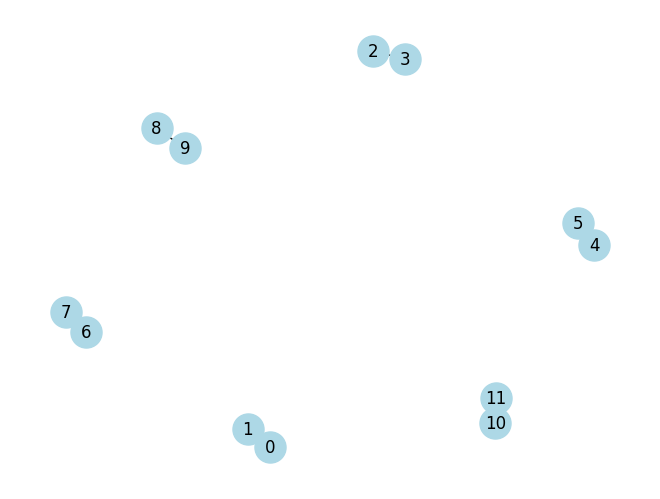
\includegraphics[width=0.6\textwidth]{figures/m_k2_graph.png}
    \caption{Visualization of the $M=6$-$K_2$ components graph.}
    \label{fig:m_k2_graph}
\end{figure}

\subsection*{Nodes within Connected Components}
For nodes within each $K_2$ component, we expect a high cosine similarity in their embeddings. \\
In a $K_2$ graph, the only possible walks are between the two connected nodes. \\
The DeepWalk algorithm, which relies on these walks to generate embeddings,
will frequently observe these two nodes in proximity. 
Consequently, their vector embeddings will be very similar,
reflecting their direct and exclusive connection in the graph.

\subsection*{Nodes in Different Connected Components}
In contrast, nodes in different $K_2$ components are expected to exhibit lower cosine similarity in their embeddings. \\
Each $K_2$ is an isolated connected component, 
implying that random walks within one $K_2$ component do not include nodes from another $K_2$ component. \\
As a result, the embeddings generated by DeepWalk will capture this lack of relation in the graph structure, 
leading to lower similarity in the vector space for nodes from different components.

In \ref{fig:m_components}, I did a quick experiments to validate this result. This reveals the relavance of the features.
Notebook is available to reproduce these experiments.


\begin{figure}[ht]
    \centering
    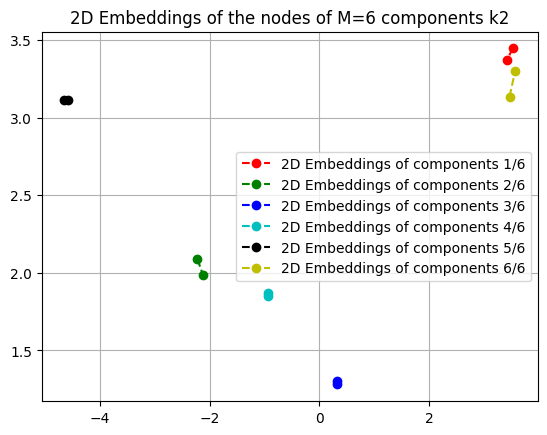
\includegraphics[width=0.6\textwidth]{figures/m_k2_graph_2d_embeddings.png}
    \caption{Relevant 2D embeddings from DeepWalk for  M-$K_2$ components. Nodes inside the same components (same color) have 
    very similar 2D embeddings whereas nodes from different components are farther away.}
    \label{fig:m_components}
\end{figure}


\section{Node classification}
\subsection*{Task 5: visualization of Zachary's karate club}

\begin{figure}[ht]
    \centering
    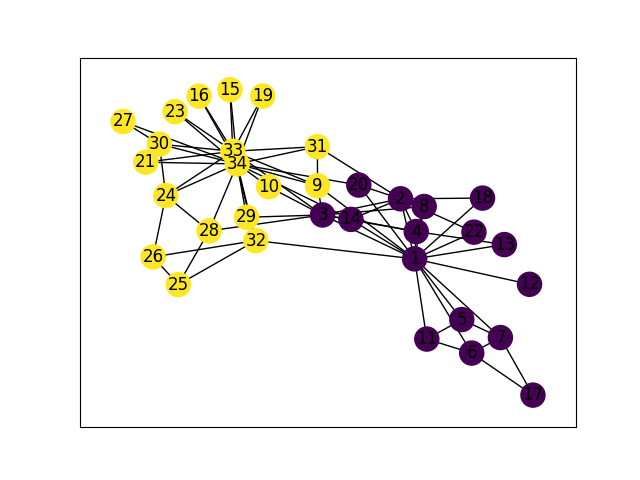
\includegraphics[width=0.5\textwidth]{figures/labeled_karate_graph.png}
    \caption{Visualization of the Karate graph with 2 labels (groundtruth)}
    \label{fig:karate_labeled}
\end{figure}

\break
\subsection*{Task 6/7/8: Classification of Zachary's karate club}
\begin{verbatim}
    Deep walk embeddings: accuracy = 1.000
    Spectral embeddings accuracy =  0.857
\end{verbatim}
These results are given for a training ratio of 80\% on a single training/validation set split. 
A more fair evaluation reveals an accuracy of 99\% with Deep walk embeddings accuracy and 79\% with Spectral embdeddings,
in average over 1000 runs, with a training data ratio of 80\%,
please refer to \ref{fig:deepwalk_vs_laplacian_embdeddings}.
\subsection*{Comparison of DeepWalk embeddings and spectral embeddings}
The code for this part can be found in \textit{code/part1/classifiers\_comparisons.py}


Unsupervised deepwalk embeddings are much more powerful than spectral embeddings when evaluated on
the weakly supervised classification task as shown on \ref{fig:deepwalk_vs_laplacian_embdeddings}.
\begin{figure}[ht]
    \centering
    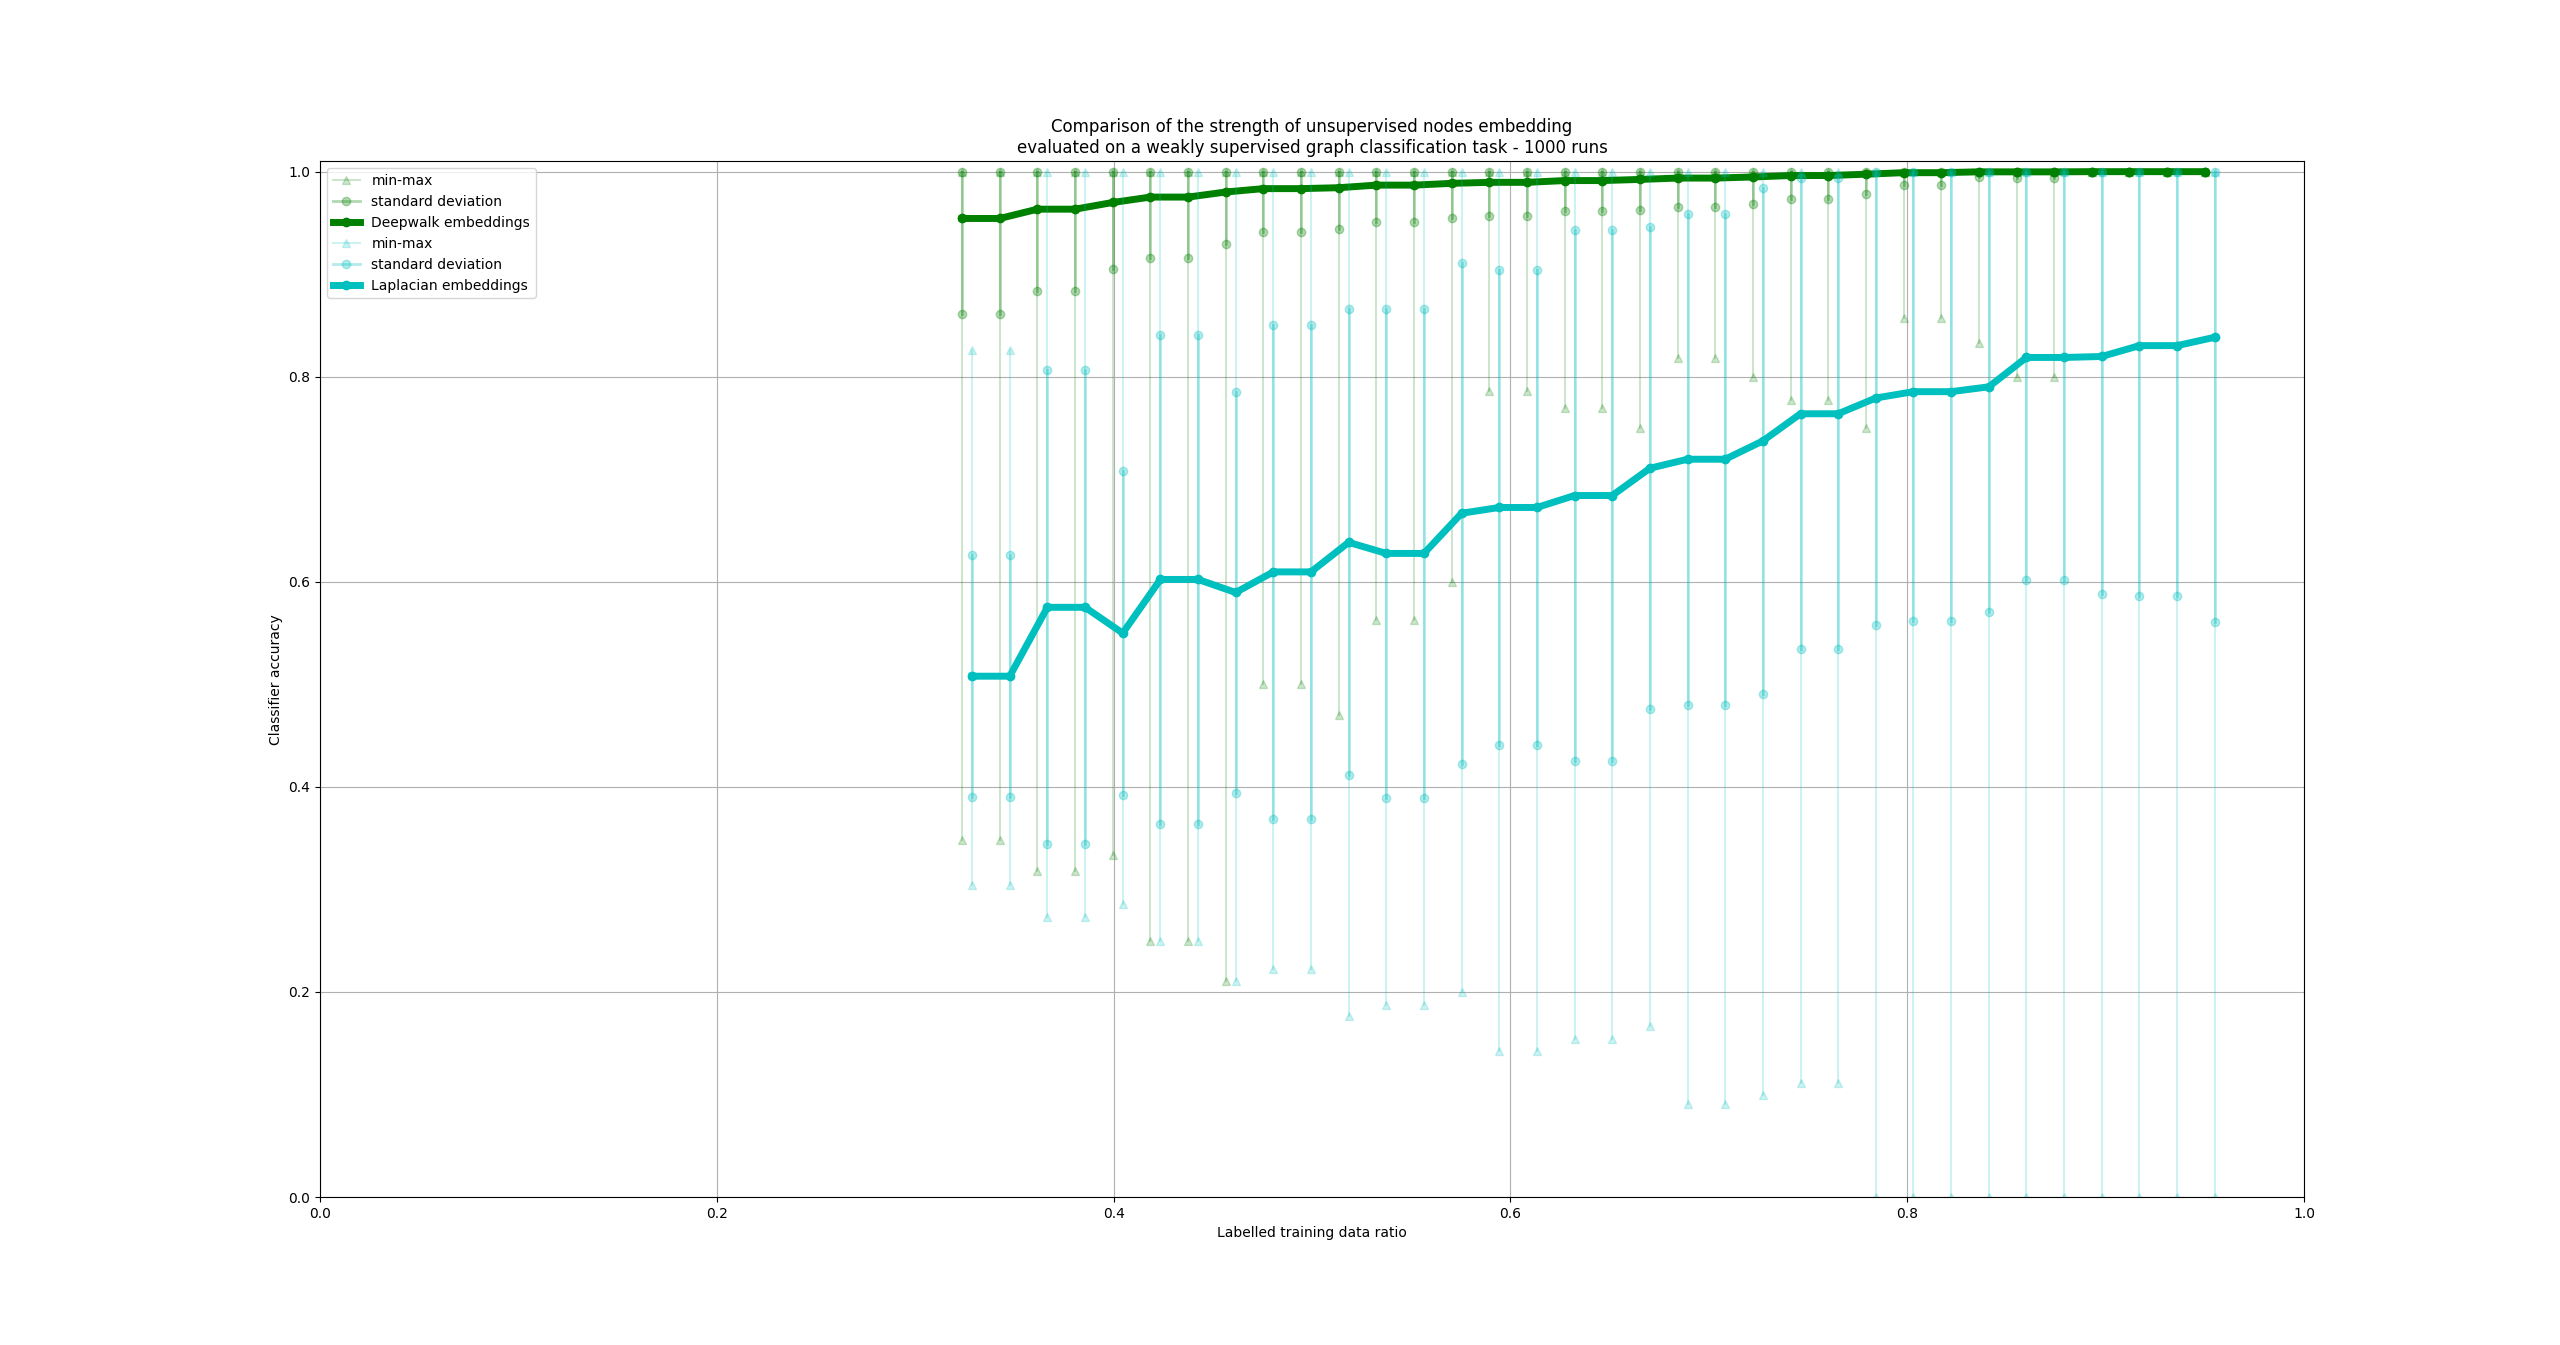
\includegraphics[width=1.\textwidth]{figures/deepwalk_vs_laplacian_embeddings_1000runs.png}
    \caption{Average classification accuracy over 1000 runs (various seeds) for various training ratios. 
    min \& max accuracy and standard deviation over the 1000 runs are reported.}
    \label{fig:deepwalk_vs_laplacian_embdeddings}
\end{figure}
\textit{Please keep in mind that as the training ratio increase, we also get less data for evaluation.
Accuracies reported for 95\% of training data leave 5\% if unlabelled data for evaluation,
thus not making a really fair job.} It is impressive to see that with only 30\% of the labels being given, deep walk
embeddings based classifier is able to classify the remaining 70\%unlabelled nodes with an accuracy of 95\%.
Spectral features give 50\% accuracy in this same regime, meaning they're nearly not informative in this case.



\break

\section{Graph Neural Networks}
\subsection*{Question 3}


We're looking at the scenario where no self-loops were added to the graph (e.g. if we'd work with the raw adjacency matrix after normalization
$D^{-\frac{1}{2}} A D^{-\frac{1}{2}}$). This is a bad idea and we'll try to explain why.
\begin{itemize}
    \item The node's hidden state is solely a function of its neighbors' features.
    \item The node's own features are not considered directly, potentially losing the unique characteristics of the node itself. This might lead to less effective representations.
\end{itemize}


\subsubsection*{Single layer case}
\hrule

Consider a single layer network, removing the self-loop makes the learning task more difficult as the node feature itself is not used, only its neighbor features are used and aggregated.
\\
\\
Take the example of the \textbf{star graph}. 
\begin{itemize}
    \item Satellite nodes become indistiguishable as they will only receive the same message from the central node. 
    \item After the first convolution layer, all satellite nodes have the same feature.
    \item Add the self-loop back and all satellite nodes are different and keep a trace of their input feature.
\end{itemize}

Intuitively, the node feature may contain unique characteristics: 
if we provide one-hot encoded vectors (like we do in task 11) as input features to a standard classifier (ignoring the graph aspects e.g. setting the adjacency graph to identity),
we could memorize most of the training graph labels at training time. Test accuracy would be low though as the graph structure is ignored.
These self loops allow passing the current node feature to the next layer.\\
Note: \textit{nn.Linear(n\_feat, n\_classes)} is able to totally overfit and memorize the training node labels when providing input features.
Putting a mix of message passing from the neighbors and this memorization ability makes a GNN sucessful.




\subsubsection*{Two layer case}
\hrule

For the star graph case
\begin{itemize}
    \item The center node will recover its original feature (as the average over all satellite nodes features which were made identical afterthe first layer).
    \item After the second convolution layer, all satellites nodes have the same feature (broadcast of the central node feature).
\end{itemize}
\subsection*{Task 11: GNN Classification on karate club - one-hot encoded input features \\ 100\% accuracy}
\begin{verbatim}
Epoch: 100 loss_train: 0.0016 acc_train: 1.0000 time: 0.0152s
Test set results: loss= 01 accuracy= 1.0000
\end{verbatim}

\subsection*{Task 12: GNN Classification on karate club - identical input features \\ 28.6\% accuracy}
\begin{verbatim}
Epoch: 100 loss_train: 0.6655 acc_train: 0.6667 time: 0.0059s
Test set results: loss= 0.7871 accuracy= 0.2857
\end{verbatim}  
\textbf{Network cannot make a distinction between the input nodes features.}

For instance, it prevents the network from memorizing a mapping between the training node "indexes" and the output class.
It inherently forces the network to recognize structure patterns from the edges to label the nodes both at training and inference time...
which makes the classification task almost impossible 
(it could work if the 2 clusters had 2 very different structures, like a star graph and a clique connected to each other with like 1 link,
there could be a chance identical features would allow classifying the 2 groups.)

In the case of on-hot encoded input features, at training time, the network can memorize that some labels correspond
to a given class and later at inference time, convolution allow to spread this information to unlabelled nodes...
wich results in far better results.



\subsection*{Task 13:Supervised GNN Classification on Cora \\ 87.1\% accuracy}
\begin{verbatim}
Epoch: 100 loss_train: 0.1436 acc_train: 0.9550 loss_val: 0.4949 acc_val: 0.8745 time: 0.0130s
Test set results: loss= 0.5189 accuracy= 0.8708
\end{verbatim}


\begin{figure}[ht]
    \centering
    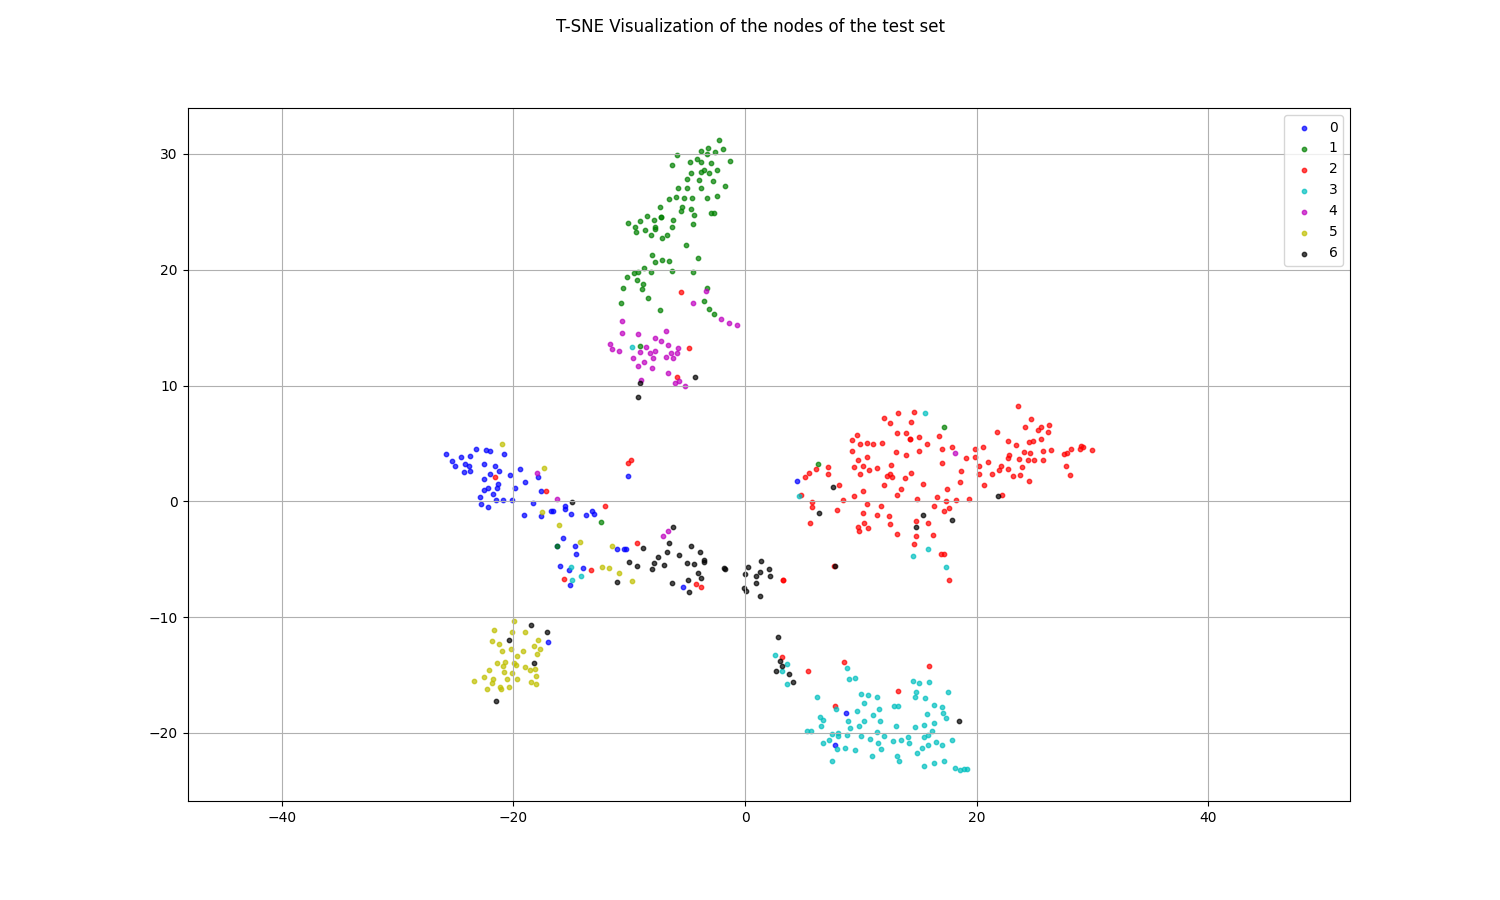
\includegraphics[width=1.\textwidth]{figures/tSNE_Cora.png}
    \caption{Visualization of the discriminative features learnt by the GNN (second hidden linear layer). 
    High dimensional $(32)$ hidden feature vectors of 542 test nodes are visualized in a low 2D dimension space using T-SNE}
    \label{fig:tsne_cora}
\end{figure}
\break
\subsection*{Question 4}
\subsection*{Methodology}

Rational approach is to use Sympy for the following computations.

Here's the example for the star graph

\begin{verbatim}
from sympy import symbols, Matrix, sqrt, Rational, latex, evaluate, N, Max

# Input features
X = Matrix([[1], [1], [1], [1]])

# First layer weights
W_0 = Matrix([[Rational(1, 2), -Rational(2, 10)]])


### STAR GRAPH
# Define the variable u
u = 1/sqrt(2)
# Normalized adjacency matrix (computed semi manually)
A = Rational(1, 2) * Matrix([
    [Rational(1, 2), u, u, u],
    [u, 1, 0, 0],
    [u, 0, 1, 0],
    [u, 0, 0, 1]
])

# First layer hidden unit
Z_0_before_relu = A*X*W_0
Z_0 = Z_0_before_relu.applyfunc(lambda x: Max(0, x))

# Second layer weights 
# Note: second row of W_1 will not be used as Z_0 second column is full of zeros
W_1 = Matrix([
    [Rational(3,10), -Rational(2,5), Rational(4,5), Rational(1,2)],
    [-1.1, 0.6, -0.1, 0.7]
])
Z_1 = (A*Z_0*W_1).applyfunc(lambda x: Max(0, x))
\end{verbatim}


\hrule
Here's an additional validation to check that the analytic expressions match with the numerical computation
\begin{verbatim}
from utils import normalize_adjacency
import networkx as nx
import numpy as np
G = nx.star_graph(3)
Anorm = normalize_adjacency(nx.adjacency_matrix(G))
X = np.ones((4, 1))
W0 = np.array([[0.5, -0.2]])
W1 = np.array([[0.3, -0.4, 0.8, 0.5], [-1.1, 0.6, -0.1, 0.7]])
Z0 = (Anorm@X@W0).clip(0, None)
Z1 = (Anorm@Z0@W1).clip(0, None)
print(f"{Z0} \n{np.array(N(Z_0))}")
print(f"{Z1} \n{np.array(N(Z_1))}")
\end{verbatim}
\hrule

\break
\subsection*{Star graph}

    
$ A_{S^4} = \begin{bmatrix}
    0  &  1  &  1  &  1 \\
    1  &  0  &  0  &  0 \\
    1  &  0  &  0  &  0 \\
    1  &  0  &  0  &  0 
\end{bmatrix}
$

$\tilde{A}_{S^4} = A_{S^4} + I = \begin{bmatrix}
    1  &  1  &  1  &  1 \\
    1  &  1  &  0  &  0 \\
    1  &  0  &  1  &  0 \\
    1  &  0  &  0  &  1 
  \end{bmatrix}
$

$ \tilde{D_{S^4}} = \text{diag}[4, 2, 2, 2] = \begin{bmatrix}
    4  &  0  &  0  &  0 \\
    0  &  2  &  0  &  0 \\
    0  &  0  &  2  &  0 \\
    0  &  0  &  0  &  2 
\end{bmatrix}$


$\tilde{D_{S^4}}^{-\frac{1}{2}} = \text{diag}[\frac{1}{2}, \frac{1}{\sqrt{2}}, \frac{1}{\sqrt{2}}, \frac{1}{\sqrt{2}}] = 
\begin{bmatrix}
    \frac{1}{2}  &  0  &  0  &  0 \\
    0  &  \frac{1}{\sqrt{2}}  &  0  &  0 \\
    0  &  0  &  \frac{1}{\sqrt{2}}  &  0 \\
    0  &  0  &  0  &  \frac{1}{\sqrt{2}} 
\end{bmatrix}$


$\hat{A_{S^4}} = \tilde{D_{S^4}}^{-\frac{1}{2}} .\tilde{A}_{S^4} .\tilde{D_{S^4}}^{-\frac{1}{2}} $





$\hat{A_{S^4}} = \begin{bmatrix}
    \frac{1}{4} &  \frac{1}{2\sqrt{2}}  &  \frac{1}{2\sqrt{2}}  &  \frac{1}{2\sqrt{2}} \\
    \frac{1}{2\sqrt{2}}  &  \frac{1}{2}  &  0 &  0\\
    \frac{1}{2\sqrt{2}}  &  0 &  \frac{1}{2}  &  0\\
    \frac{1}{2\sqrt{2}}  &  0 &  0 &  \frac{1}{2} 
\end{bmatrix} =
\left[\begin{matrix}\frac{1}{4} & \frac{\sqrt{2}}{4} & \frac{\sqrt{2}}{4} & \frac{\sqrt{2}}{4}\\\frac{\sqrt{2}}{4} & \frac{1}{2} & 0 & 0\\\frac{\sqrt{2}}{4} & 0 & \frac{1}{2} & 0\\\frac{\sqrt{2}}{4} & 0 & 0 & \frac{1}{2}\end{matrix}\right]
\approx \begin{bmatrix}
    0.25 &  0.354 &  0.354 &  0.354\\
    0.354 &  0.5 &  0 &  0\\
    0.354 &  0 &  0.5 &  0\\
    0.354 &  0 &  0 &  0.5
\end{bmatrix}
$

Let's use $u := \frac{1}{\sqrt{2}}$

$\hat{A_{S^4}}.X. W^{0} = \frac{1}{4}\begin{bmatrix}
    \frac{1}{2} + 3u &  -? \\
    u+1 &  -? \\
    u+1 &  -? \\
    u+1 &  -? \\
\end{bmatrix}$

$Z^{0} = \begin{bmatrix}
    \frac{1}{2} + 3u & 0 \\
    u+1 &  0 \\
    u+1 &  0 \\
    u+1 &  0 \\
\end{bmatrix}
$


I used the $?$ symbol to skip computation because there's no need to perform this computation since these are negative numbers
which will be zeroed by $f=\text{ReLU}$


$Z^{0} = \left[\begin{matrix}\frac{1}{8} + \frac{3 \sqrt{2}}{8} & 0\\\frac{\sqrt{2}}{8} + \frac{1}{4} & 0\\\frac{\sqrt{2}}{8} + \frac{1}{4} & 0\\\frac{\sqrt{2}}{8} + \frac{1}{4} & 0\end{matrix}\right]
\approx \begin{bmatrix}
    0.655 &  0\\
    0.427 &  0\\
    0.427 &  0\\
    0.427 &  0
  \end{bmatrix}
$


To compute $Z^{1}$, we have to nottice straight away that the second row of $W^{1}$ will be multiplied only by $0$

$W^{1} = \left[\begin{matrix}\frac{3}{10} & - \frac{2}{5} & \frac{4}{5} & \frac{1}{2}\\-1.1 & 0.6 & -0.1 & 0.7\end{matrix}\right]$

Performing computation manually does not make sense here and the room for mistake is huge.
We use symbolic calculus to perform the computation correctly.

$\hat{A_{S^4}}.Z^{0}. W^{1} = 
\left[\begin{matrix}\frac{3}{320} + \frac{9 \sqrt{2}}{320} + \frac{9 \sqrt{2} \left(\frac{\sqrt{2}}{8} + \frac{1}{4}\right)}{40} & - \frac{3 \sqrt{2} \left(\frac{\sqrt{2}}{8} + \frac{1}{4}\right)}{10} - \frac{3 \sqrt{2}}{80} - \frac{1}{80} & \frac{1}{40} + \frac{3 \sqrt{2}}{40} + \frac{3 \sqrt{2} \left(\frac{\sqrt{2}}{8} + \frac{1}{4}\right)}{5} & \frac{1}{64} + \frac{3 \sqrt{2}}{64} + \frac{3 \sqrt{2} \left(\frac{\sqrt{2}}{8} + \frac{1}{4}\right)}{8}\\\frac{3 \sqrt{2}}{160} + \frac{3}{80} + \frac{3 \sqrt{2} \cdot \left(\frac{1}{8} + \frac{3 \sqrt{2}}{8}\right)}{40} & - \frac{\sqrt{2} \cdot \left(\frac{1}{8} + \frac{3 \sqrt{2}}{8}\right)}{10} - \frac{1}{20} - \frac{\sqrt{2}}{40} & \frac{\sqrt{2}}{20} + \frac{1}{10} + \frac{\sqrt{2} \cdot \left(\frac{1}{8} + \frac{3 \sqrt{2}}{8}\right)}{5} & \frac{\sqrt{2}}{32} + \frac{1}{16} + \frac{\sqrt{2} \cdot \left(\frac{1}{8} + \frac{3 \sqrt{2}}{8}\right)}{8}\\\frac{3 \sqrt{2}}{160} + \frac{3}{80} + \frac{3 \sqrt{2} \cdot \left(\frac{1}{8} + \frac{3 \sqrt{2}}{8}\right)}{40} & - \frac{\sqrt{2} \cdot \left(\frac{1}{8} + \frac{3 \sqrt{2}}{8}\right)}{10} - \frac{1}{20} - \frac{\sqrt{2}}{40} & \frac{\sqrt{2}}{20} + \frac{1}{10} + \frac{\sqrt{2} \cdot \left(\frac{1}{8} + \frac{3 \sqrt{2}}{8}\right)}{5} & \frac{\sqrt{2}}{32} + \frac{1}{16} + \frac{\sqrt{2} \cdot \left(\frac{1}{8} + \frac{3 \sqrt{2}}{8}\right)}{8}\\\frac{3 \sqrt{2}}{160} + \frac{3}{80} + \frac{3 \sqrt{2} \cdot \left(\frac{1}{8} + \frac{3 \sqrt{2}}{8}\right)}{40} & - \frac{\sqrt{2} \cdot \left(\frac{1}{8} + \frac{3 \sqrt{2}}{8}\right)}{10} - \frac{1}{20} - \frac{\sqrt{2}}{40} & \frac{\sqrt{2}}{20} + \frac{1}{10} + \frac{\sqrt{2} \cdot \left(\frac{1}{8} + \frac{3 \sqrt{2}}{8}\right)}{5} & \frac{\sqrt{2}}{32} + \frac{1}{16} + \frac{\sqrt{2} \cdot \left(\frac{1}{8} + \frac{3 \sqrt{2}}{8}\right)}{8}\end{matrix}\right]$

We nottice that the second column is filled with negative numbers.

$Z^{1} = f(\hat{A_{S^4}}.Z^{0}. W^{1}) =  \left[\begin{matrix}\frac{3}{320} + \frac{9 \sqrt{2}}{320} + \frac{9 \sqrt{2} \left(\frac{\sqrt{2}}{8} + \frac{1}{4}\right)}{40} & 0 & \frac{1}{40} + \frac{3 \sqrt{2}}{40} + \frac{3 \sqrt{2} \left(\frac{\sqrt{2}}{8} + \frac{1}{4}\right)}{5} & \frac{1}{64} + \frac{3 \sqrt{2}}{64} + \frac{3 \sqrt{2} \left(\frac{\sqrt{2}}{8} + \frac{1}{4}\right)}{8}\\\frac{3 \sqrt{2}}{160} + \frac{3}{80} + \frac{3 \sqrt{2} \cdot \left(\frac{1}{8} + \frac{3 \sqrt{2}}{8}\right)}{40} & 0 & \frac{\sqrt{2}}{20} + \frac{1}{10} + \frac{\sqrt{2} \cdot \left(\frac{1}{8} + \frac{3 \sqrt{2}}{8}\right)}{5} & \frac{\sqrt{2}}{32} + \frac{1}{16} + \frac{\sqrt{2} \cdot \left(\frac{1}{8} + \frac{3 \sqrt{2}}{8}\right)}{8}\\\frac{3 \sqrt{2}}{160} + \frac{3}{80} + \frac{3 \sqrt{2} \cdot \left(\frac{1}{8} + \frac{3 \sqrt{2}}{8}\right)}{40} & 0 & \frac{\sqrt{2}}{20} + \frac{1}{10} + \frac{\sqrt{2} \cdot \left(\frac{1}{8} + \frac{3 \sqrt{2}}{8}\right)}{5} & \frac{\sqrt{2}}{32} + \frac{1}{16} + \frac{\sqrt{2} \cdot \left(\frac{1}{8} + \frac{3 \sqrt{2}}{8}\right)}{8}\\\frac{3 \sqrt{2}}{160} + \frac{3}{80} + \frac{3 \sqrt{2} \cdot \left(\frac{1}{8} + \frac{3 \sqrt{2}}{8}\right)}{40} & 0 & \frac{\sqrt{2}}{20} + \frac{1}{10} + \frac{\sqrt{2} \cdot \left(\frac{1}{8} + \frac{3 \sqrt{2}}{8}\right)}{5} & \frac{\sqrt{2}}{32} + \frac{1}{16} + \frac{\sqrt{2} \cdot \left(\frac{1}{8} + \frac{3 \sqrt{2}}{8}\right)}{8}\end{matrix}\right]$
$Z^{1}  \approx \begin{bmatrix}
    0.185 &  0 &  0.493 &  0.308\\
    0.134 &  0 &  0.356 &  0.223\\
    0.134 &  0 &  0.356 &  0.223\\
    0.134 &  0 &  0.356 &  0.223
\end{bmatrix}$

% \bibliographystyle{plain}
% \bibliography{references} % citation records are in the references.bib document

\end{document}